\documentclass[12pt]{article}
\usepackage{geometry}
\geometry{a4paper}
\usepackage[sort,comma]{natbib}
\usepackage{graphicx}
\usepackage[T1]{fontenc}
\usepackage[utf8]{inputenc}
\usepackage{textcomp}
\usepackage{gensymb}
\usepackage{amsmath}
\usepackage{amssymb}
\usepackage{authblk}
\usepackage[running]{lineno}
\usepackage{setspace}
\usepackage{rotating}
\usepackage{pdflscape}
\usepackage[most]{tcolorbox}

\doublespacing


\title{\large \texttt{insectDisease}: programmatic access to the \textit{Ecological Database of the World's Insect Pathogens}}

\renewcommand\Authfont{\fontsize{12}{14.4}\selectfont}
\renewcommand\Affilfont{\fontsize{10}{10.8}\itshape}

\author[a,b,*]{Tad A Dallas}
\author[c]{Colin Carlson}

% \author[c]{David Onstad}




\affil[a]{Department of Biological Sciences, Louisiana State University, Baton Rouge, LA, USA}
\affil[b]{Department of Biological Sciences, University of South Carolina, Columbia, SC, USA}

\affil[c]{  }
\affil[d]{  }



\renewcommand\Authands{ and }
 \date{ \small *Corresponding author: tad.a.dallas@gmail.com}






%%% Target journal
% Ecography (software note)
%
%


%%% Potential reviewers
% 
% 
% 
% 


%%% Editors
% Thiago Rangel
% 
% 



\begin{document}
\maketitle
\setstretch{1}

\vspace{-1cm}
\noindent \textbf{Author contributions}: TAD developed the R package, with taxonomic functions developed by CC. All authors contributed to manuscript writing.  \\

\noindent \textbf{Acknowledgements}: We sincerely thank all individuals associated with the collection and curation of the \textit{Ecological Database of the World's Insect Pathogens} data, specifically David Onstad at the US Department of Agriculture. \\

\noindent \textbf{Conflict of interest}: The authors have no conflicts of interest to declare. \\

\noindent \textbf{Keywords}: insect pathogens, crop pest, experimental infection,   \\


\clearpage
\setstretch{1.35}
\linenumbers


\subsection*{Abstract}



















\medskip

\noindent \textbf{Running title}: Ecological Database of the World's Insect Pathogens (EDWIP)  \\














\clearpage
\setstretch{1.9}
\section*{Introduction}


% the lack of insect disease data
There are a number of data sources documenting host-pathogen associations, especially for pathogens of mammals \citep{gibb2021, patrick2017}, birds \citep{bensch2009}, and fish \citep{fishpest}. These have been incredibly important to our understanding of what determines pathogen host range, pathogen species richness across a set of hosts, and overall host-pathogen network structure (e.g, \citep{dallas2018, carlson2020}). But while some host groups are well-studied, there are taxonomic gaps in our understanding of host-pathogen associations. For instance, insect host-pathogen relationships have considerably less open-source data available, despite their inherent importance to agricultural crops and vector-borne disease, in addition to the numerical dominance of insect species over other taxa \citep{stork2015}. This is a clear knowledge gap. 






% the file drawer issue and
\paragraph*{}
Additionally, all of the previous data sources listed before have dedicated researchers and government agencies responsible for data deposition and curation in openly accessible formats. However, some data have not been as lucky, at no fault of the original data curators. These data run the risk of disappearing into a file drawer or on an external hard drive, potentially shared with a small number of researchers but not accessible to the scientific community at large. One data resource arguably close to this point of disappearance is the \textit{Ecological Database of the World's Insect Pathogens} (EDWIP) \citep{onstad1997}. 



% edwip
\paragraph*{}
The EDWIP data consist of experimental infections and field observations of the interactions between insect hosts and a number of nematode, viral, protozoan, fungal, and bacterial pathogens \citep{braxton2003}. In the EDWIP data, a number of pathogen infection types were excluded, including vector-borne pathogens which do not infect the insect host. An interesting component of EDWIP is the existence of negative associations -- attempts to inoculate a host with a given pathogen that failed to infect -- for some host groups (Figure \ref{fig:bubble}). Failed infections represent \textit{true} absences or incompatibilities between a given host and pathogen. These data are incredibly useful to pathogen host range and host-pathogen interaction modeling, but we rarely have data on these known non-interactions. Initially created in 1996, the data have been dynamically updated over time. However, it is unclear how long this curation continued, and how many different versions of the data may be in existence without proper versioning. To this point, the numbers of insect-host pathogen interactions differs slightly from previously published versions of the data \citep{braxton2003}, but these changes are relatively minor. 



\subsection*{Solution statement}

To preserve these data in a format that is well-documented, openly accessible, versioned, and flexible for continued development, we created the \texttt{insectDisease} R package. In doing so, we implicitly adhere to the FAIR (Findable, Accessible, Interoperable, Resuable) guidelines for managing data. By hosting the data openly on GitHub, and versioning releases of the data with a permanent identifier (DOI), we ensure the longevity and versioned curation of this data resource. Finally, the incorporation of taxonomic data through \texttt{taxize} \citep{chamberlain2013} makes sure that host and pathogen taxonomic names are updated. 


















\subsection*{Data specification}

% Discuss more of the in-depth view of the R package as a means for data delivery, and what the overall workflow looks like. Discuss how it's open and all part of the Verena ecosystem (or whatever). Flex on data size and point to figures displaying the positive and negative associations and such. 


\paragraph*{Package structure}

Data products are broken down by pathogen group; nematodes (\texttt{data(nematode)}), viruses (\texttt{data(viruses)}), and non-viral pathogens, which include protozoan, fungi, and bacteria (\texttt{data(nvpassoc)}). Data on negative associations is stored collectively instead of being delineated by pathogen group (\texttt{data(negative)}), but information on pathogen group is provided within each of these files, allowing for sorting of negative interactions based on the initial pathogen groupings. 


\paragraph*{}
Each of the pathogen groups slightly differs in the available data on experimental infections. For instance, nematode infections contain information on soil type and associated bacteria, virus infection data has information on viral dose, and non-viral pathogens (protozoans, fungi, and bacteria) have information on intermediate host species.


\paragraph*{}
Data are also available on the insect host species themselves (e.g., \texttt{?hosts} or \texttt{data(hosts)}). These data contain some information on Canadian province where the host is found (\texttt{ProvinceI} column), what it eats (\texttt{Food} column), and what type of habitat it is found in (\texttt{Habitat} column). Additionally, a column on host insect pest status is present, offering the opportunity to explore study effort and pathogen specificity dependent on the pest status of the insect host. 











\paragraph*{Metadata and package documentation}

Differences in features across the data on different pathogen types (e.g., \texttt{?nematodes} relative to \texttt{?viruses}) make combining these data difficult without a loss of information. However, there is clear utility in having all of the data in a single standardized form. As such, we have documented each data resource using R package documentation, allowing the metadata of each data product to be examined directly from R using the \texttt{help()} function or the question mark notation (e.g., \texttt{?viruses}). 














\paragraph*{Data cleaning and taxonomic resolution}

The initial data structure was maintained from the original raw data files provided by David Onstad, principal maintainer of the EDWIP data resource \citep{onstad1997}. This includes files such as \texttt{new\_assoc}, as this was likely a test file containing pathogen species such as "wormy thing". We clean and augment this existing data source programmatically, with much of this code in the \texttt{insectDisease} package \texttt{vignette}. 



\paragraph*{}
First, we resolve host and pathogen names using the R package \texttt{taxize}, using NCBI taxonomic backbone \citep{chamberlain2013}. While this seems like a small change, it both standardizes host and pathogen nomenclature, and catches any taxonomic changes that have occurred in the past couple decades. This includes the consideration of microsporidian parasites as fungi, not protozoans, a change affecting a large set of records in the EDWIP data. Second, we provide a vignette which combines the different host-pathogen data together to form an informative set of host-pathogen associations, including both both known associations and failed experimental infections, as delineated by the \texttt{interaction} column in the resulting \texttt{edwip.csv} file. Finally, processed data by the vignette is output in \texttt{.csv} format in the vignettes folder, but all data stored as R data objects (\texttt{.rda}) are also converted to csv and placed in the \texttt{csv} folder, allowing non-R users to still access the data in a stable format. 





















\subsection*{Case study: covariance among pathogen groups in parasite species richness }

Hosts that are infected by more pathogens of one type may also be more infected by pathogens of another type, mediated by host life history traits, metabolic demands, geographic distribution, and intensity of scientific study \citep{dallas2021}. We explore this in the EDWIP data by measuring the number of known positive associations of each of the pathogen groups for each insect host species, visualizing the relationship between the number of pathogens per insect host as a correlation matrix (Figure \ref{fig:corPlot}). We find very little evidence that pathogen groups have positive covariance, which would be expected if host species traits drove infection process across pathogen groups in the same manner. The failure to detect positive relationships, and indeed some negative relationships appearing, could be a signal of the targeted nature of data collection, as many insect host species were selected to study due to their potential as a crop pest, and many pathogens were selected to study based on their potential use as biocontrol or perhaps for their ease of culture. 

\paragraph*{}
This potential sampling bias among insect host species would be clear if there were a positive relationship between the number of positive interactions to the number of negative interactions for a host species, as it would indicate that insect host species with lots of known interactions also tended to appear in many studies and have some negative interactions as well. We find evidence for a significantly negative relationship based on a Spearman's rank correlation ($\rho$ = -0.1, p $<$ 0.0001). 





















\subsection*{Concluding comments}

Ecological data -- while growing in availability, size, and stability -- are still a resource that should not be allowed to fade out of existence. The EDWIP data provided to the authors were in a proprietary format ('Claris FileMaker Pro 5') that was already over 10 major versions behind. With limited inter-version operability (e.g., \texttt{.fmp5} files cannot be opened in more recent versions of the software, or require multiple conversion steps), these data seemed as if headed towards obsolescence. The \texttt{insectDisease} package ensures that these data will be available to the broadest set of researchers, be bound to relevant metadata, and be properly versioned. By hosting the data openly, we welcome contributions from researchers interested in augmenting the data or building off the existing resource. 







\subsection*{Data accessibility}

The \texttt{insectDisease} R package is currently available on GitHub https://github.com/viralemergence/insectDisease, with '.csv' files in the csv directory for long-term data stability. 

Finally, the data are periodically archived at major version changes via Zenodo ?????????????????? 
 















\clearpage
\bibliography{var}
\bibliographystyle{ecography}
\clearpage


























\clearpage

%----------------
\section*{Figures}

\begin{figure}[h!]
  \begin{center}
    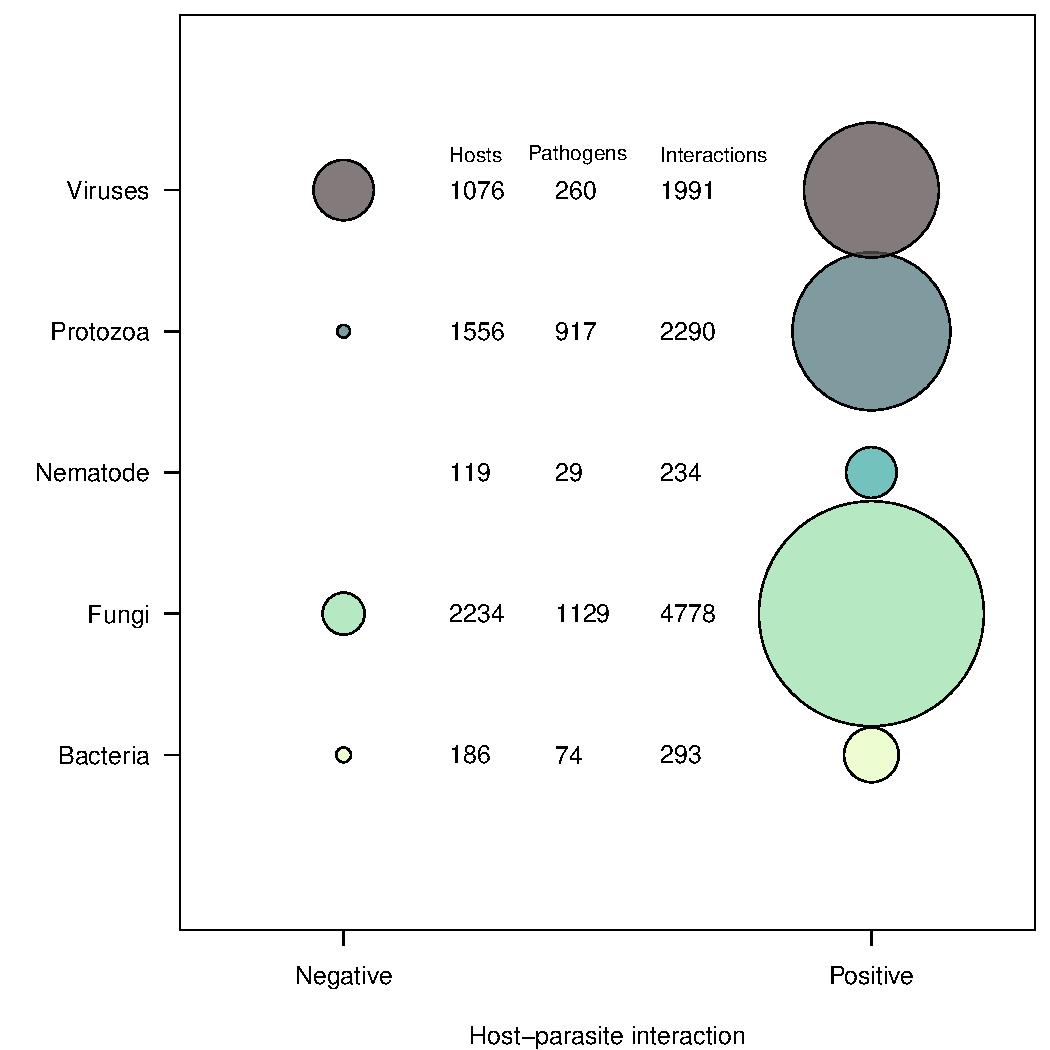
\includegraphics[width=0.85\textwidth]{Figures/bubble.pdf}
    \caption{Bubble plot, where points are proportional to the total number of negative (on the left) and positive (on the right) host-pathogen interactions for each pathogen group ($y$-axis). Numeric columns correspond to the number of unique host species, pathogen species, and interactions for each pathogen group. }
    \label{fig:bubble}
  \end{center}
\end{figure}




\clearpage


\begin{figure}[h!]
  \begin{center}
    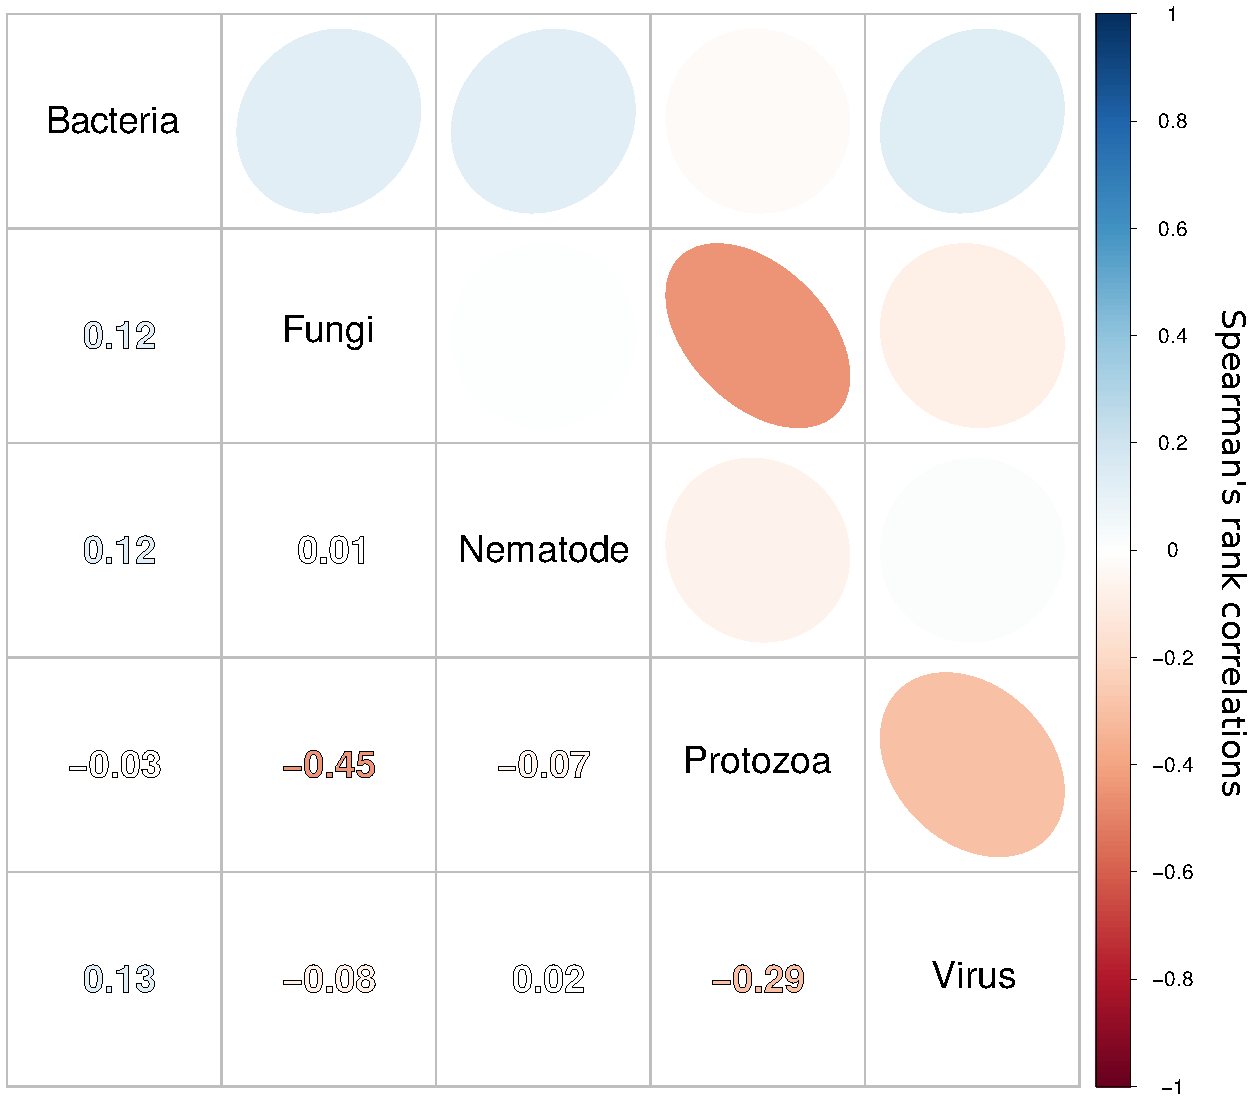
\includegraphics[width=0.8\textwidth]{Figures/corPlot.pdf}
    \caption{Correlations between each pathogen group in terms of pathogen richness of insect host species, where color corresponds to Spearman's rank correlation values (provided in the lower diagonal matrix). Fungal and protozoan pathogens seemed to negatively covary, as did viruses and protozoans. Understanding to what extent this is driven by sampling effects or insect host ecology is an outstanding research question that these could be used to begin addressing.}
    \label{fig:corPlot}
  \end{center}
\end{figure}






\end{document}
